\documentclass[a4paper,12pt]{article}

% ---------- Packages ----------
\usepackage[a4paper,margin=1in]{geometry}
\usepackage{fancyhdr}
\usepackage{xcolor}
\usepackage{graphicx}
\usepackage{float}
\usepackage{amsmath}
\usepackage{listings}
\usepackage{hyperref}
\begin{document}
\pagestyle{fancy}
\fancyhf{}
\fancyhead[L]{
\includegraphics[height=1cm]{IIITB-COMET-Logo.png}}
\fancyhead[R]{Name: P.Muskan\\ID: cometfwc035}

\section*{Question}
\begin{figure}[H]
 \centering
 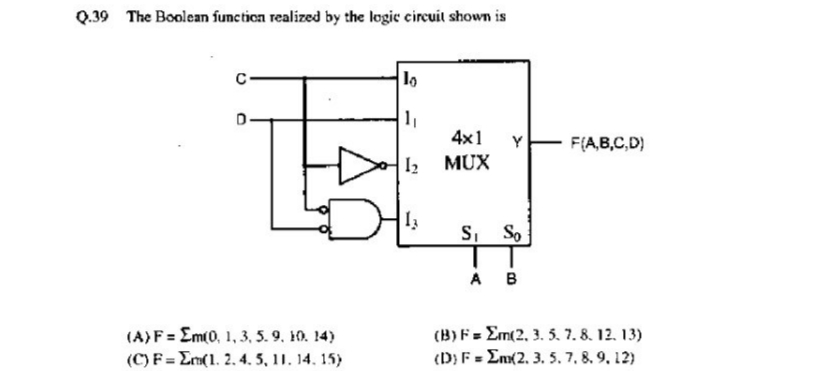
\includegraphics[width=0.8\linewidth]{question.jpg}
\end{figure}
% ---------- Code Style ----------
\lstdefinestyle{verilog}{
  language=Verilog,
  backgroundcolor=\color{gray!10},
  basicstyle=\ttfamily\footnotesize,
  frame=single,
  keywordstyle=\color{blue},
  commentstyle=\color{gray},
  numbers=left,
  numberstyle=\tiny\color{gray},
  breaklines=true,
  showstringspaces=false,
  captionpos=b
}

% ---------- Document ----------

\begin{center}
    \Huge\textbf{Implementation of 4x1 Multiplexer using Verilog and Vaman Board}\\[1em]
    \Large\textbf{Hardware Implementation Report}\\[1em]
\end{center}
\section*{Q.1 FPGA  Experiment}
\section*{Objective}
To design, simulate, and physically implement a 4x1 multiplexer using Verilog HDL on a Vaman FPGA development board. The output of the multiplexer is observed using LEDs.

\section*{Hardware Required}
\begin{itemize}
    \item Vaman FPGA Board
    \item LEDs
    \item Resistors (220 $\Omega$)
    \item Jumper Wires
    \item Breadboard
\end{itemize}

\section*{Theory}
A multiplexer (MUX) is a combinational circuit that selects one of several input signals and forwards the selected input to a single output line.  
A 4x1 multiplexer has 4 input lines, 2 selection lines, and 1 output line.

The truth table for a 4x1 MUX is as follows:

\begin{center}
\begin{tabular}{|c|c|c|}
\hline
Select Lines (S1 S0) & Selected Input & Output (Y) \\
\hline
00 & I0 & I0 \\
01 & I1 & I1 \\
10 & I2 & I2 \\
11 & I3 & I3 \\
\hline
\end{tabular}
\end{center}

\section*{Verilog Code}
\begin{lstlisting}[style=verilog, caption={4x1 Multiplexer Verilog Code}]
module mux4x1(
    input I0, I1, I2, I3,
    input S0, S1,
    output reg Y
);
always @(*) begin
    case ({S1, S0})
        2'b00: Y = I0;
        2'b01: Y = I1;
        2'b10: Y = I2;
        2'b11: Y = I3;
    endcase
end
endmodule
\end{lstlisting}

\section*{PCF File (Pin Constraint File)}
\begin{lstlisting}[style=verilog, caption={.pcf File for Vaman Board Pin Mapping}]
set_io I0  J15  # Switch 1
set_io I1  L16  # Switch 2
set_io I2  M13  # Switch 3
set_io I3  R15  # Switch 4
set_io S0  P14  # Select Line 1
set_io S1  N16  # Select Line 2
set_io Y   K13  # LED Output
\end{lstlisting}

\section*{Procedure}
\begin{enumerate}
    \item Write the Verilog code for a 4x1 multiplexer.
    \item Create a new project in the Vaman IDE or through command line using Yosys and nextpnr.
    \item Add the Verilog file and PCF file to the project.
    \item Synthesize and implement the design.
    \item Generate the bitstream or binary (.bin) file.
    \item Upload the bitstream to the Vaman board.
    \item Connect LEDs and switches to observe the multiplexer output.
\end{enumerate}

\section*{Output and Observation}
When the select lines are changed, the output LED glows corresponding to the selected input line as per the truth table.

\section*{Conclusion}
The 4x1 multiplexer was successfully implemented on the Vaman FPGA board. The output matched the expected behavior as per the truth table. This experiment demonstrates how combinational logic can be implemented on FPGA hardware using Verilog HDL.

\section*{Result}
A 4x1 MUX was designed, simulated, and verified on the Vaman FPGA board using LEDs as output indicators.

\end{document}
